\documentclass[10.5pt]{article}   %11 puntos

%Adapted from Adapted from UWA Engineering Final Year Project.


\usepackage[utf8]{inputenc}
\usepackage[x11names,dvipsnames,svgnames,table]{xcolor}

% general incantations
\usepackage[export]{adjustbox}
\usepackage{afterpage}

\usepackage{graphicx}
\usepackage{placeins}
\usepackage{pdfpages}
\usepackage{algorithm2e}
\usepackage{array}
\usepackage{booktabs}
\usepackage[most]{tcolorbox}
\usepackage{calligra}
\usepackage{caption}
\usepackage{datetime}
\usepackage{dirtytalk}
\usepackage{dsfont}
\usepackage{etex}
\usepackage{fancyhdr}
\usepackage{fix-cm}
\usepackage[T1]{fontenc}
\usepackage{textcomp,gensymb} %for \degree C symbol
\usepackage{graphicx}
\usepackage{lipsum}
\usepackage{listings}
\usepackage{transparent}
\usepackage[everyline=true,framemethod=tikz]{mdframed}
\usepackage{mparhack}
\usepackage{multicol}
\usepackage{multirow}
\usepackage{parskip}
\usepackage{lscape}
\usepackage{pdflscape}
\usepackage{pdfpages}
\usepackage{placeins}
\usepackage[document]{ragged2e}
\usepackage{rotating}
\usepackage{setspace}
\usepackage{subcaption}
\usepackage{threeparttable}
\usepackage[normalem]{ulem}
\usepackage{verbatim}
\usepackage{soul} %highlighting, strike through etc.

%Automated appendices
\usepackage[titletoc,title,header]{appendix} %advanced functionality

%language settings
\usepackage[utf8]{inputenc}
\usepackage{csquotes}

%page setup
%this where we adjust the binding offset, if relevant
\usepackage{geometry}
\geometry{left=2cm,right=2cm,top=2cm,bottom=2cm}
\usepackage{lastpage} % for page 1 of n footers

%cross referencing
\usepackage[hidelinks]{hyperref}
\usepackage{cleveref}

%maths stuff
\usepackage{amsmath}
\usepackage{mathtools}

\setcounter{secnumdepth}{5}

%lists
\usepackage{enumitem}

%working collaboratively
\usepackage[backgroundcolor=yellow]{todonotes}

% bibliography file using harvard
\usepackage[style=apa,citestyle=bwl-FU,backend=biber, sorting=nyt]{biblatex}
\bibliography{bibliography.bib} % with extension

%glossary for acronyms
\usepackage[acronym,nonumberlist,toc,section=subsection,numberedsection=nolabel]{glossaries} 
\makeglossaries

%line spacing
\linespread{1.6}


\usepackage{times}                      %Times New Roman
\usepackage{setspace}                   %Para espaciar
%\linespread{1.25}                      %Interlineado 1.5
%\singlespacing                          %Espaciado simple

\newcommand*\Heq{\ensuremath{\overset{\kern2pt LH }{=}}}
\newcommand{\Lagr}{\mathcal{L}}         %L (lagrangiano o fun de verosimilitud)
\newcommand{\indep}{\rotatebox[origin=c]{90}{$\models$}}
\newcommand{\R}{\mathbb{R}}             %Real numbers
\usepackage[utf8x]{inputenc}
%\usepackage{apacite}                    %Citas tipo apa
%\renewcommand{\thesubsection}{\thesection.\alph{subsection}}
%\usepackage{cite}
%\usepackage[left=2.5cm,right=2.5cm,top=2.5cm,bottom=2.5cm]{geometry} %Deberían ser 3 y 3 los left y right pero lo hago así para que entre mejor
%\usepackage[round]{natbib}              %Bibliografía
%\usepackage[utf8]{inputenc}
%\usepackage{amsmath}
\usepackage{mathtools}                  %Loads amsmath
\usepackage{amssymb}

\numberwithin{equation}{section}
\usepackage{hyperref}
\usepackage{color}   %May be necessary if you want to color links
 \hypersetup{
     colorlinks=false, %set true if you want colored links
     linktoc=all,     %set to all if you want both sections and sections linked
     linkcolor=blue,  %choose some color if you want links to stand out
 }
 \usepackage[spanish,es-tabla]{babel}
 \usepackage{graphicx}
 \usepackage{physics}
 %\usepackage[hidelinks]{hyperref}

\usepackage{amssymb}    %Para tener los check mark y cruces
\usepackage{pifont}     %Para tener los check mark y cruces
\newcommand{\cmark}{\ding{51}} %Para tener los check mark y cruces
\newcommand{\xmark}{\ding{55}}  %Para tener los check mark y cruces
\usepackage{float}

%Esto lo podés volar
% \usepackage{xcolor}                 %Night mode
% \pagecolor[rgb]{0,0,0} %black       %Night mode
% \color[rgb]{0.8,0.8,0.8} %grey      %Night mode

\title{Trabajo final}
\author{Matías Harari y Mariana Santi}
\date{2° trimestre 2021}
\setlength{\marginparwidth}{2cm}
%\usepackage[utf8]{inputenc}
\usepackage{setspace}
\spacing{1.2}
\usepackage{listings}
\usepackage{color}
%\usepackage{apacite}
\usepackage{biblatex}


\definecolor{dkgreen}{rgb}{0,0.6,0}
\definecolor{gray}{rgb}{0.5,0.5,0.5}
\definecolor{mauve}{rgb}{0.58,0,0.82}

\lstset{frame=tb,
  language=Java,
  aboveskip=3mm,
  belowskip=3mm,
  showstringspaces=false,
  columns=flexible,
  basicstyle={\small\ttfamily},
  numbers=none,
  numberstyle=\tiny\color{gray},
  keywordstyle=\color{blue},
  commentstyle=\color{dkgreen},
  stringstyle=\color{mauve},
  breaklines=true,
  breakatwhitespace=true,
  tabsize=3
}

\begin{document}
\renewcommand{\thesubsection}{\thesection.\alph{subsection}}

\thispagestyle{empty}
\setlength\headheight{0pt} 
\begin{center}

\begin{center}

\includegraphics[width=0.65\linewidth]{imgs/logoudesa.png}            
\end{center}	

        \vspace{0.2cm}
        {\scshape\LARGE Departamento de Economía \par}
        \vspace{0.2cm}
        {\scshape\Large Maestría en Economía\par}
        \vspace{0.4cm}

        {\Large\bfseries Herramientas computacionales - Trabajo final}
        
        \vspace{1cm}
        {\Large\itshape Matias Harari y Mariana Santi \par}


\vspace{1cm} 
\large
{2021}

\end{center}

\clearpage
\justify
\section*{Presentación}
En un reconocido trabajo, \cite{nunn2011potato} encuentran un efecto significativo de la introducción de la papa en el Viejo Mundo sobre la explosión del crecimiento poblacional en los siglos XVIII y XIX.


En este artículo utilizamos la información abierta del apéndice online del trabajo para presentar algunos de sus resultados de una forma visualmente más creativa y llamativa. Siguiendo a \cite{schwabish2014economist}, creemos que la capacidad de motivar al lector y facilitar la comprensión de resultados es fundamental en la investigación académica contemporánea.  
\section*{Sobre la presentación del problema: la idoneidad de la papa en el Viejo Mundo}
La Figura \ref{fig1} replica el único mapa presentado en \cite{nunn2011potato}, ahora a color. Allí puede verse que, en base al \textit{Suitability Index} de la FAO, Europa tiene muy buenas condiciones para la producción de secano de papa blanca. Le modificamos la leyenda ya que las categorías discretas eran difíciles de diferenciar.

\begin{figure}[H]
\centering
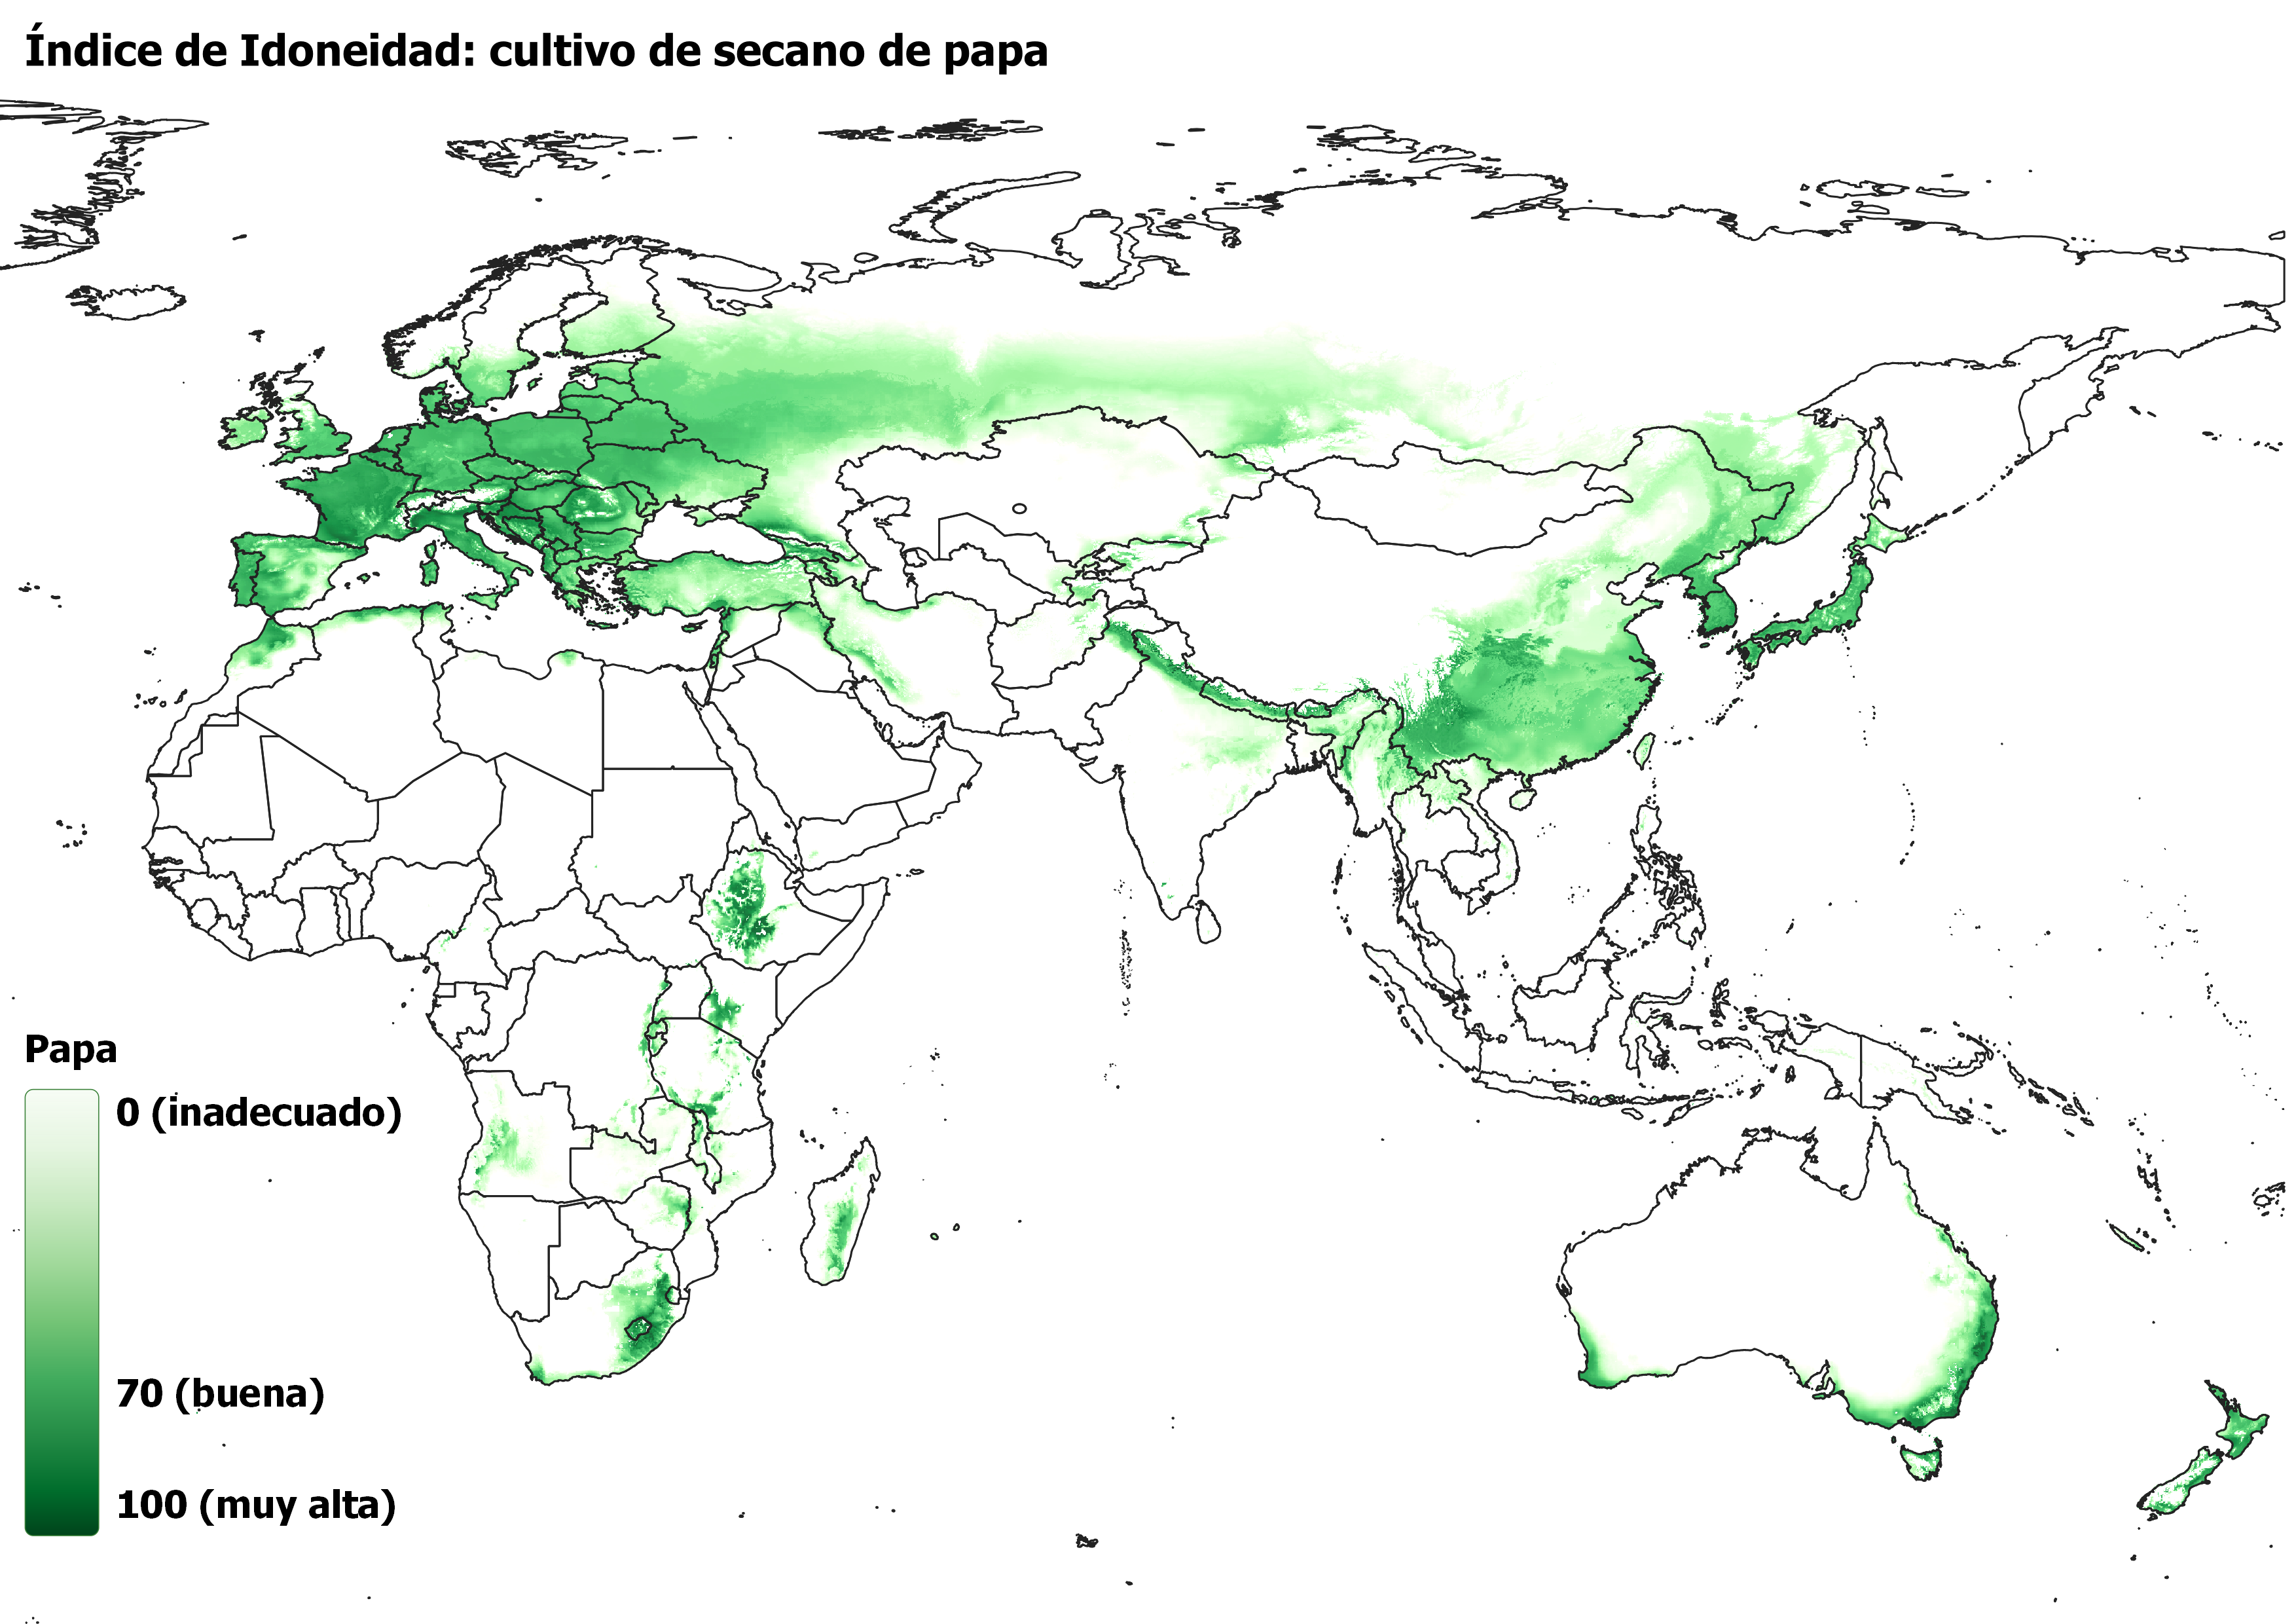
\includegraphics[scale=0.6]{imgs/wpot.png}
\caption{Índice de Idoneidad de la FAO para el cultivo de papa blanca por píxel de 0,5 x 0,5 grados.}
    \label{fig1}
\end{figure}

A grandes rasgos, la Figura \ref{fig1} no es mucho más que una gran mancha verde en Europa. Creemos que este mapa es poco representativo acerca del mensaje que quieren transmitir los autores, es decir, cómo la papa funcionó como una solución a la falta de buenos alimentos, principalmente en algunas regiones de Europa.  

Es sabido que la papa es muy idónea en casi toda Europa. Sin embargo, es menos obvio cuál fue el rol de la papa en la capacidad de alimentación de las poblaciones. Es decir, el efecto de la introducción de la papa fue mayor en aquellas regiones que no contaban con buenas condiciones para producir otros alimentos calóricos tales como el trigo, el principal alimento europeo. 
Siguiendo esta idea, la  Figura \ref{fig2} introduce a la papa como sustituto en regiones sin buenas condiciones para producir trigo. De allí puede inferirse que, probablemente, la papa fue mucho más importante en la Península Ibérica, Europa del Este y en los países del Mar del Norte que en Europa Central, donde las condiciones para producir trigo eran ideales.  

\begin{figure}[H]
\centering
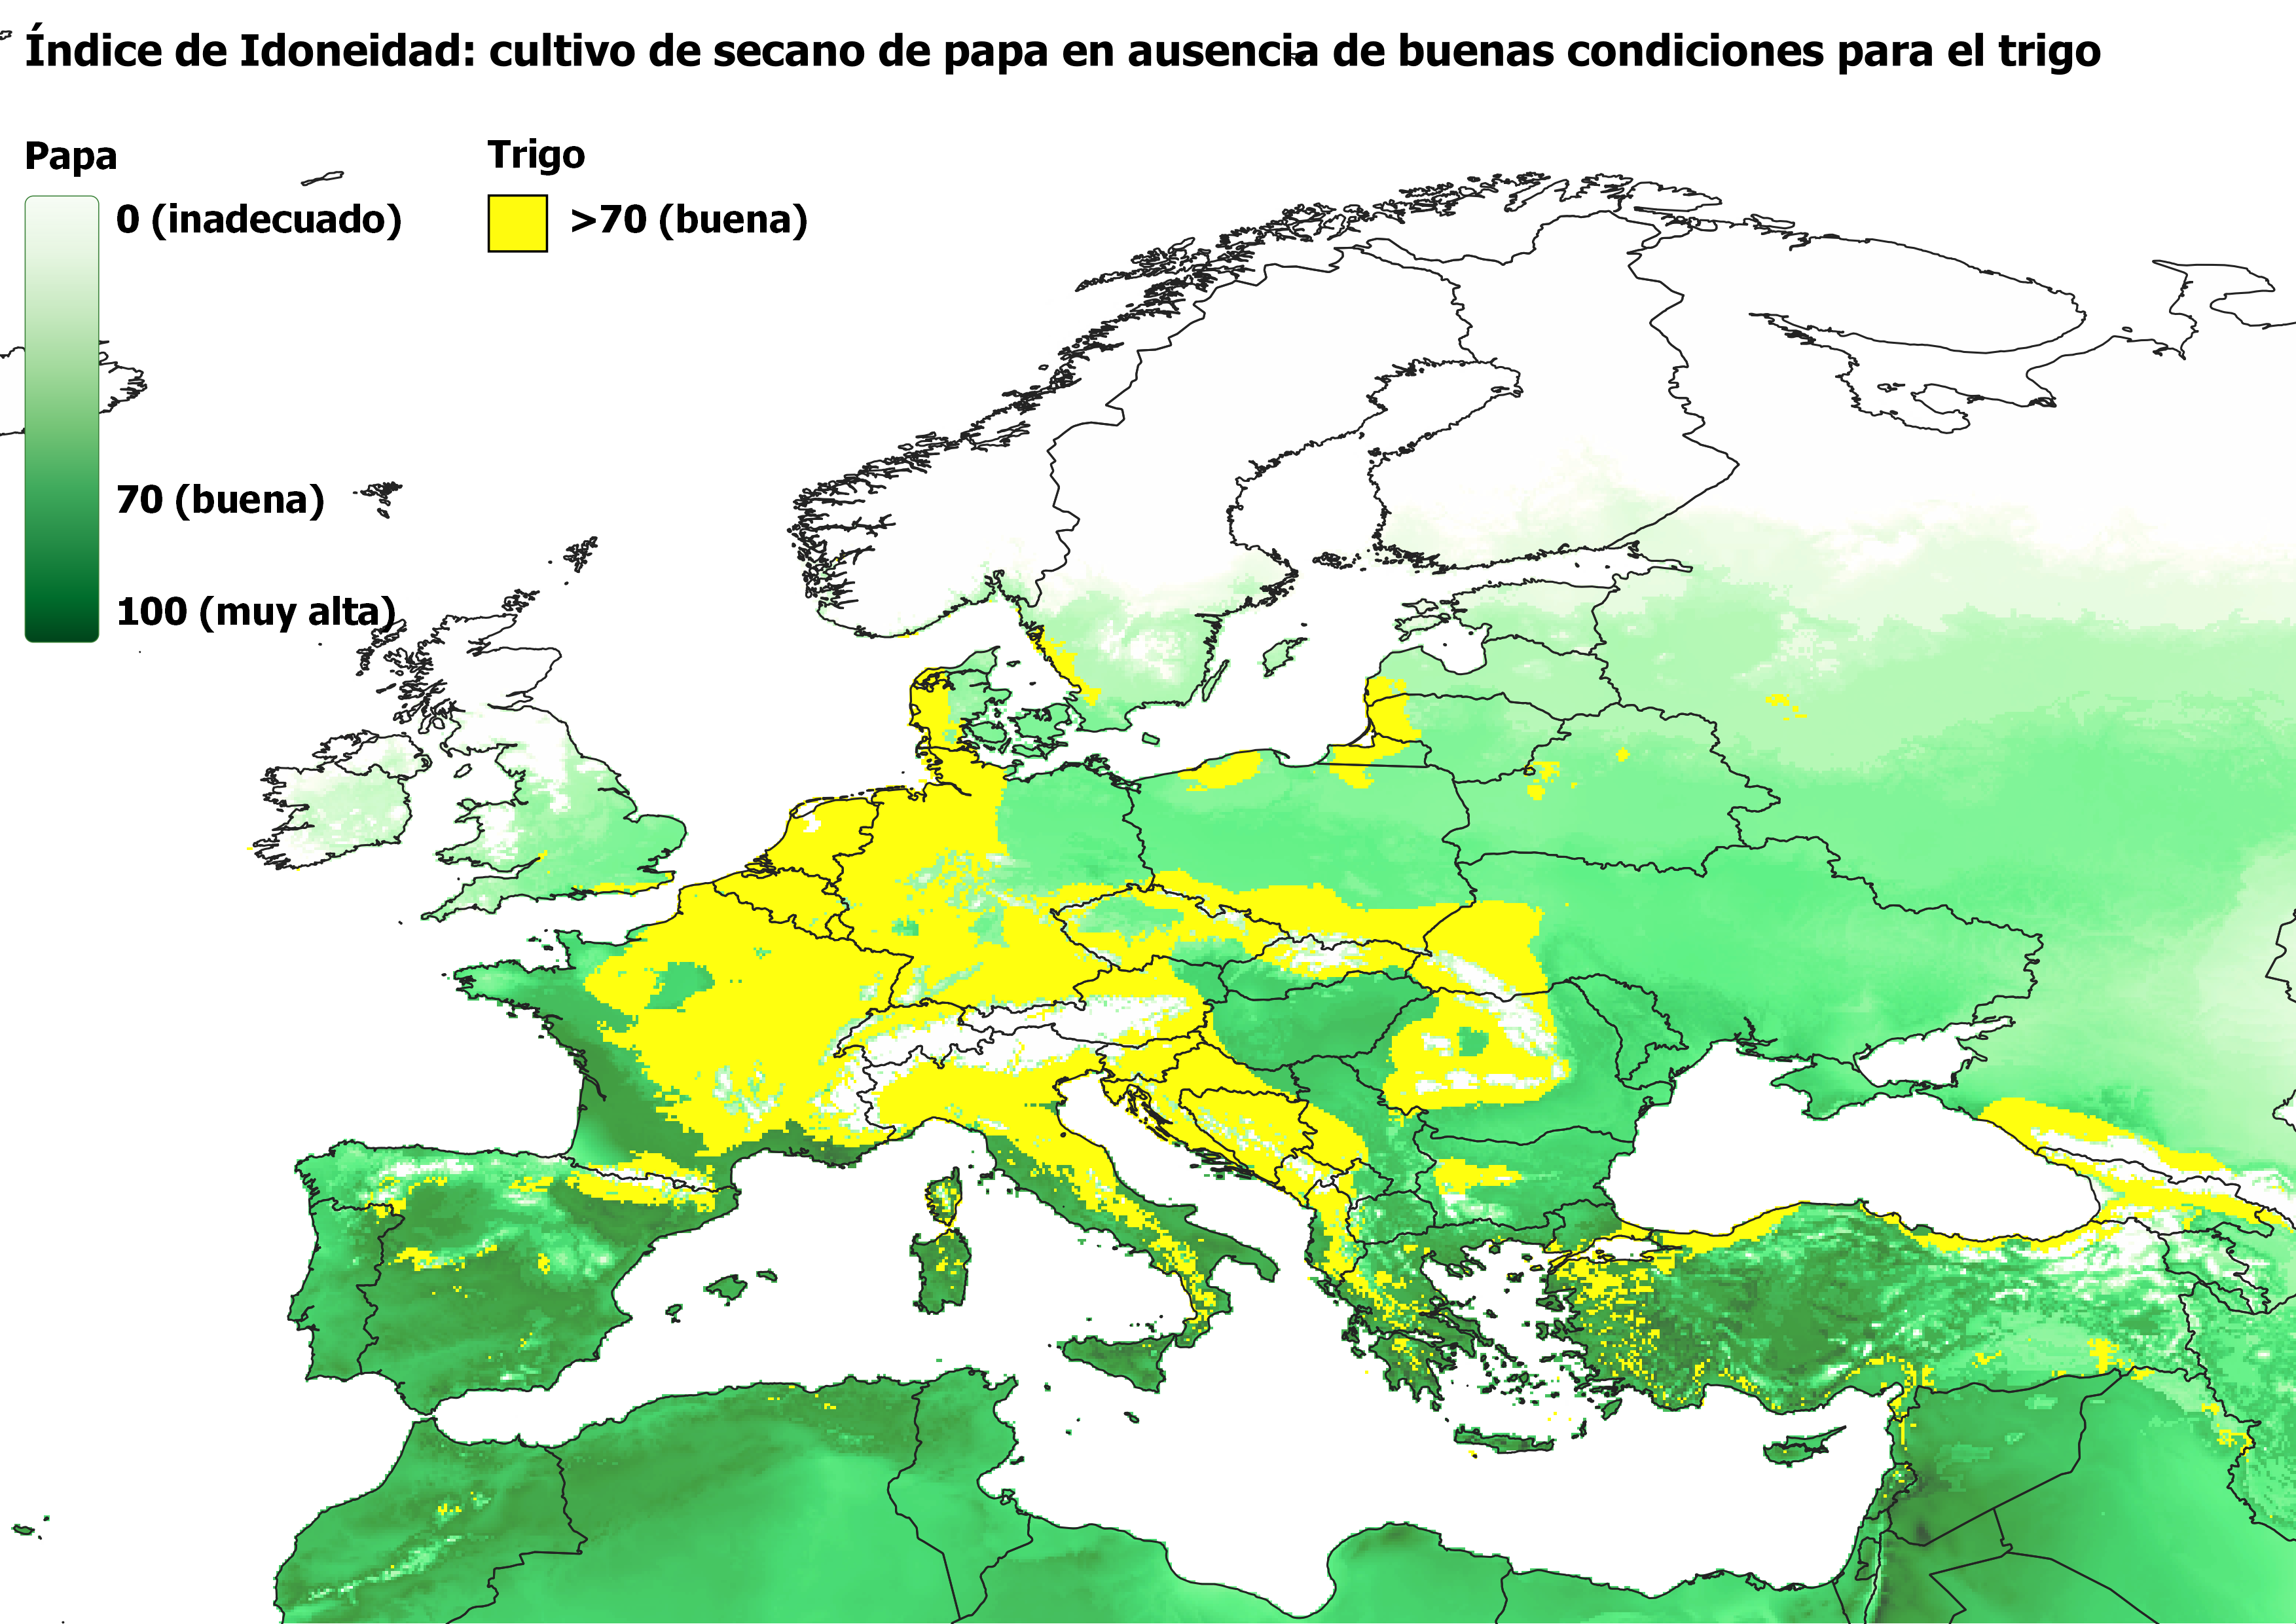
\includegraphics[scale=0.6]{imgs/wpot_wheat.png}
\caption{Índice de Idoneidad de la FAO para el cultivo de papa blanca por píxel de 0,5 x 0,5 grados. En amarillo solo se incluyeron aquellos píxeles que tenían una idoneidad alta o muy alta para el cultivo de secano de trigo.}
    \label{fig2}
\end{figure}


\section*{Sobre la conclusión principal: el efecto de la papa en el crecimiento poblacional}
Los autores encuentran un efecto causal de la idoneidad para el cultivo de papa en el Viejo Mundo sobre el incremento de la población. Para ilustrar esta relación presentamos la Figura \ref{fig3}, un mapa bivariado del Viejo Mundo que muestra la relación a nivel país entre Índice de la idoneidad de la tierra para el cultivo de papa ya mencionado y la variación de la población entre los años 1800 y 1600. Ambas fechas años se eligieron en base a la investigación de \cite{nunn2011potato}, quienes explican que en durante ese intervalo se introdujo la papa en la mayoría de las culturas del Viejo Mundo.



\begin{figure}[H]
\centering
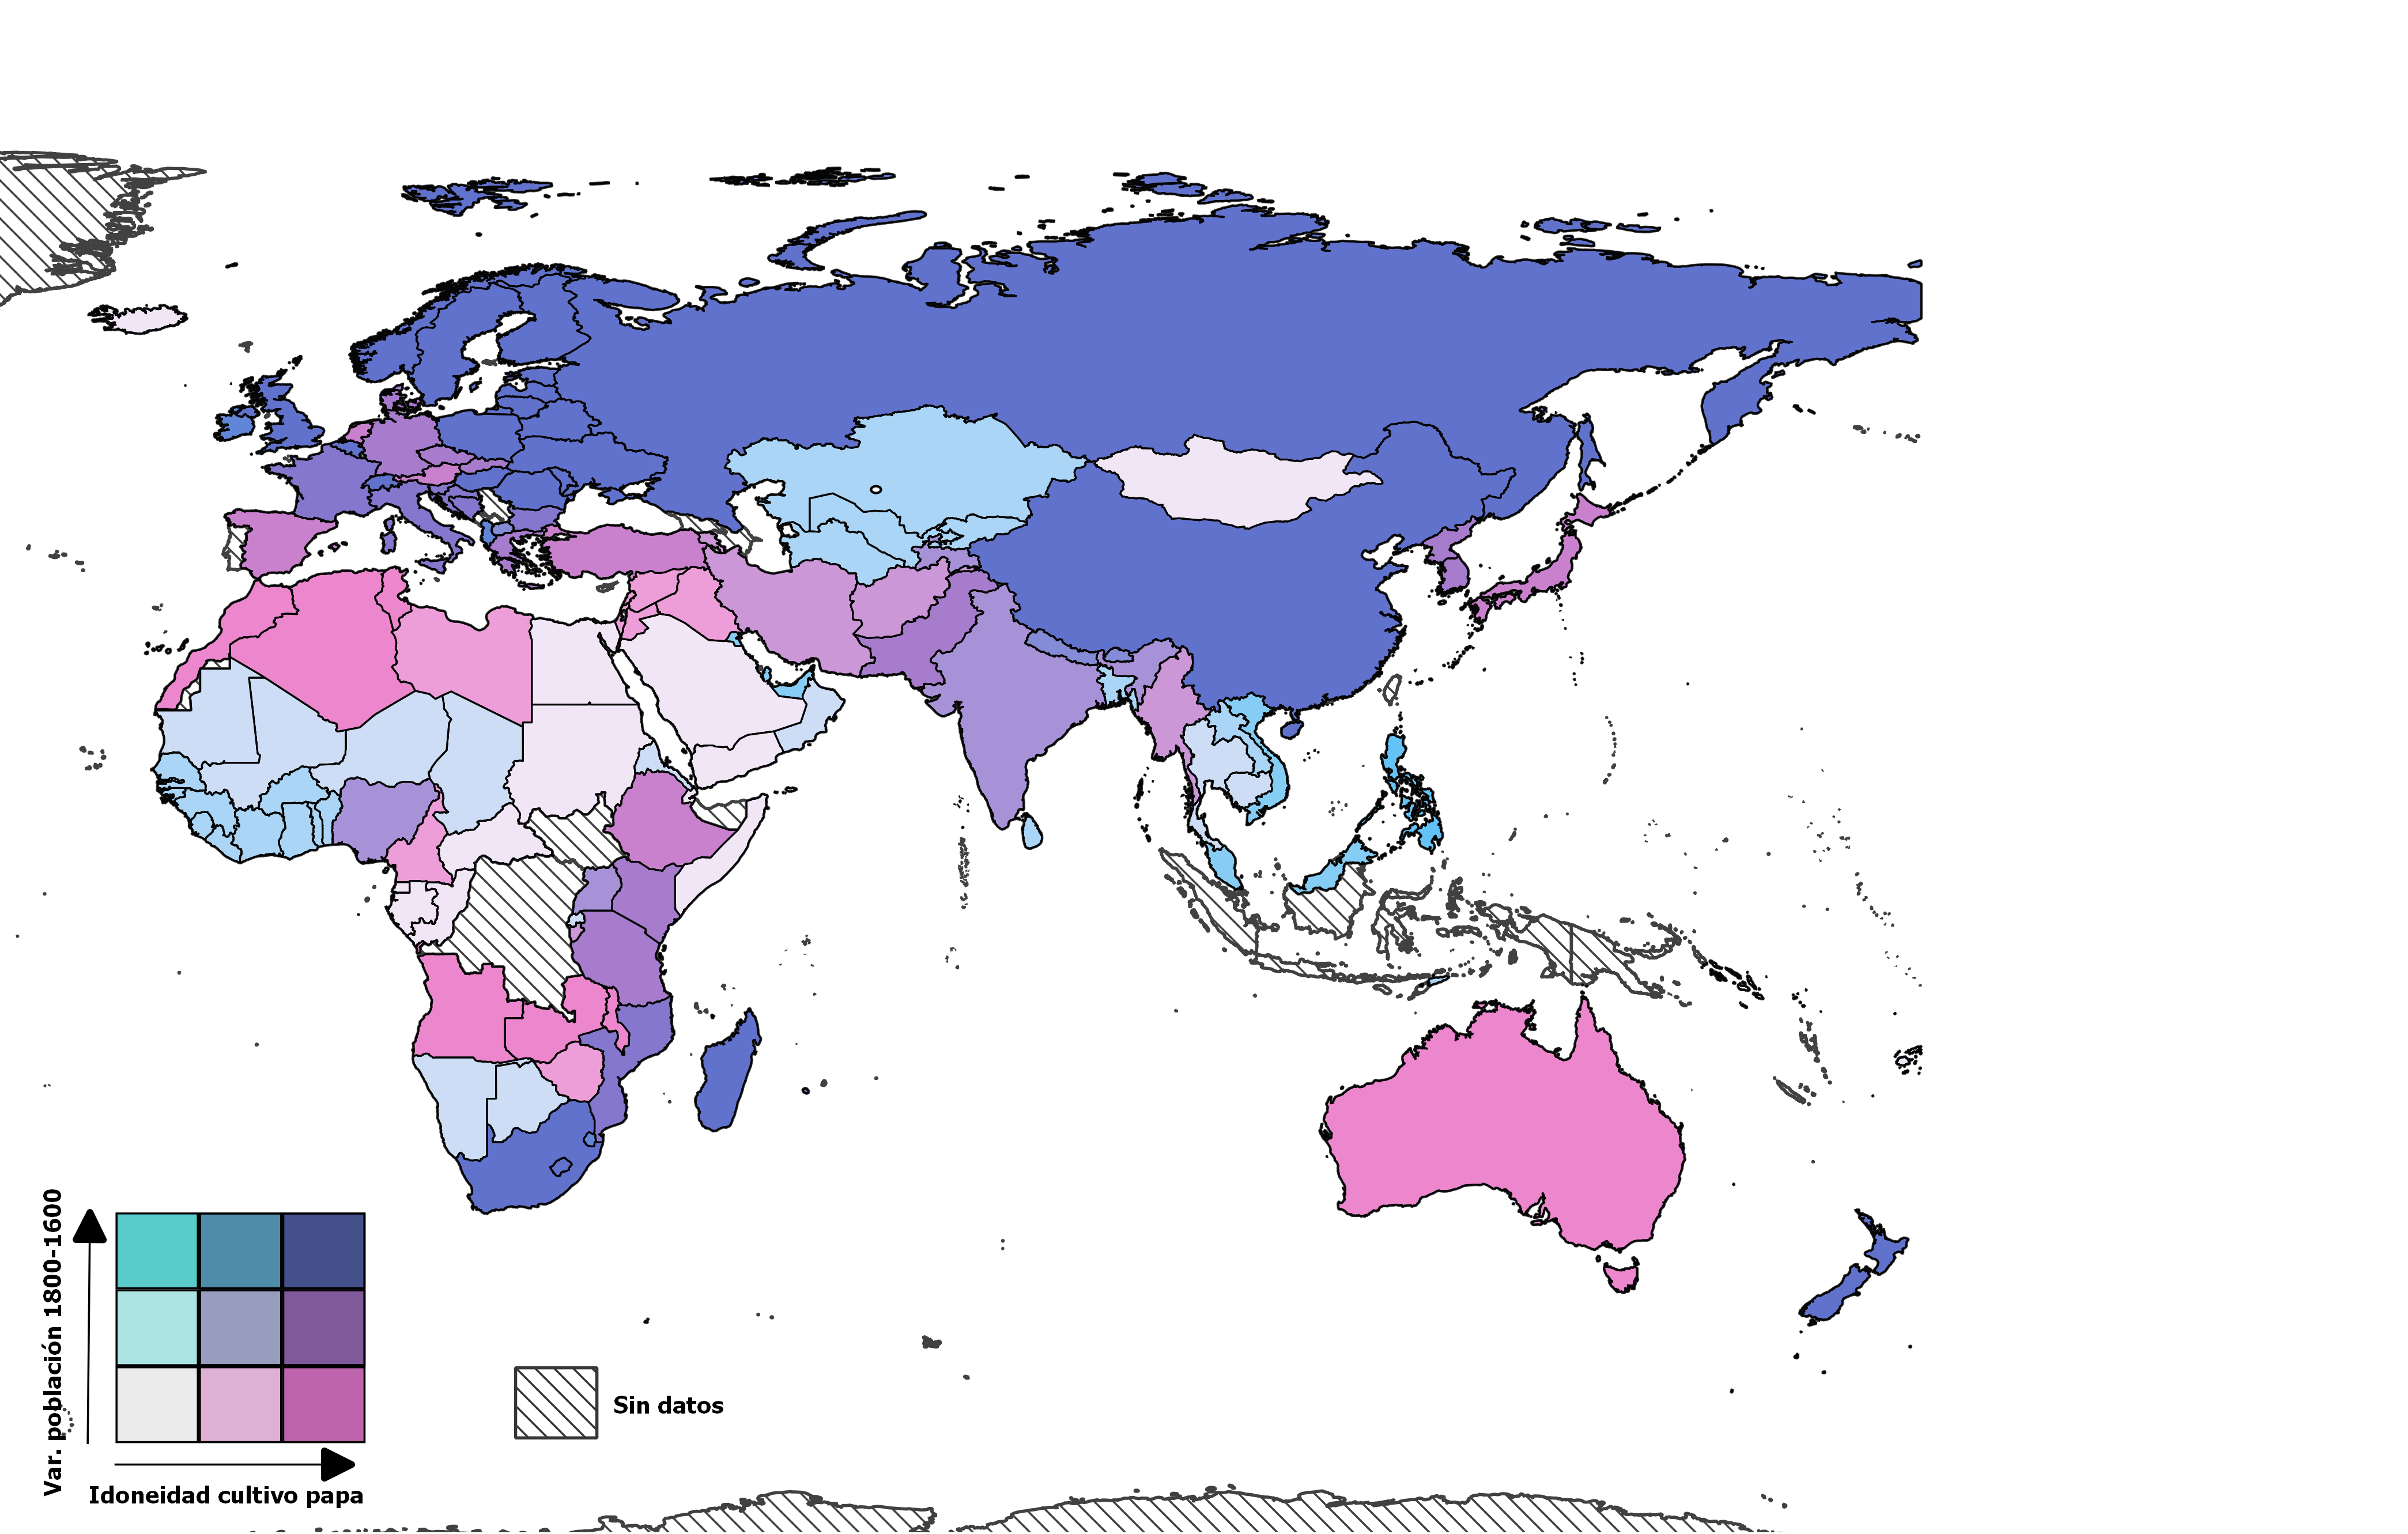
\includegraphics[scale=0.6]{imgs/Map_bivariado_var_pob y papa_v2.png}
\caption{Idoneidad para el cultivo de papa y variación de la población entre 1600 y 1800 por país}
    \label{fig3}
\end{figure}

Se puede observar que, en general, los países de mayor idoneidad para el cultivo de papa experimentaron un mayor incremento de la población. Sin embargo, existen múltiples casos donde no se observa una relación positiva entre las variables, razón por la cual \cite{nunn2011potato} introducen una serie de variables de control. Por ejemplo, Australia es idónea pero fue colonizada por Inglaterra recién en 1770, por lo que naturalmente no pudo haber existido introducción de la papa. Otro caso llamativo es el de los países mediterráneos de África, donde seguramente factores culturales e institucionales evitaron que la papa potenciara el crecimiento poblacional.

\section*{Fuentes y aclaraciones}
Para realizar el trabajo se utilizaron las bases de datos presentadas por los autores, \footnote{Ver https://scholar.harvard.edu/nunn/pages/data-0}, a excepción de los datos raster del índice de idoneidad del cultivo de papa que no estaban disponibles. En este caso, se buscó directamente la fuente utilizada por los autores (FAO gaez).\footnote{Ver ttps://gaez.fao.org/pages/data-viewer.} Los datos pueden descargarse a nivel píxel de 0,5x0,5 grados. Siguiendo el trabajo de los autores, se seleccionó cultivo de secano y no de irrigación para el año 1990.
 Los datos pueden descargarse a nivel píxel de 0,5x0,5 grados. Siguiendo el trabajo de los autores, se seleccionó cultivo de secano y no de irrigación.

%\section*{Bibliografía}
%\bibliographystyle{apacite}
\printbibliography
    
\end{document}